%#BIBTEX jbibtex results
\documentclass[final,5p,times,twocolumn]{elsarticle}
%% if you use PostScript figures in your article
%% use the graphics package for simple commands
\usepackage{graphics}
%% or use the graphicx package for more complicated commands
%% \usepackage{graphicx}
%% or use the epsfig package if you prefer to use the old commands
%% \usepackage{epsfig}

%% The amssymb package provides various useful mathematical symbols
\usepackage{amssymb}
\usepackage{amsmath}
%% The amsthm package provides extended theorem environments
%% \usepackage{amsthm}

%% The lineno packages adds line numbers. Start line numbering with
%% \begin{linenumbers}, end it with \end{linenumbers}. Or switch it on
%% for the whole article with \linenumbers after \end{frontmatter}.
%% \usepackage{lineno}

\usepackage{latexsym}
\usepackage{supertabular}
\usepackage{slashed}
\usepackage{booktabs}
\usepackage{cases}
\usepackage{bigints}
\biboptions{sort&compress}
%% natbib.sty is loaded by default. However, natbib options can be
%% provided with \biboptions{...} command. Following options are
%% valid:

%%   round  -  round parentheses are used (default)
%%   square -  square brackets are used   [option]
%%   curly  -  curly braces are used      {option}
%%   angle  -  angle brackets are used    <option>
%%   semicolon  -  multiple citations separated by semi-colon
%%   colon  - same as semicolon, an earlier confusion
%%   comma  -  separated by comma
%%   numbers-  selects numerical citations
%%   super  -  numerical citations as superscripts
%%   sort   -  sorts multiple citations according to order in ref. list
%%   sort&compress   -  like sort, but also compresses numerical citations
%%   compress - compresses without sorting
%%
%% \biboptions{comma,round}

% \biboptions{}
%%% global definitions %%%%
\newcommand{\nn}{\nonumber}
\newcommand{\simlt}{\lower.5ex\hbox{$\; \buildrel < \over \sim \;$}}

%%% local definitions %%%
\newcommand{\dsol}{\Delta_{21}}
\newcommand{\ddsol}{2\Delta_{21}}
\newcommand{\drct}{\Delta_{31}}
\newcommand{\ddrct}{2\Delta_{31}}
\newcommand{\datm}{\Delta_{32}}
\newcommand{\ssol}{\sin^22\theta_{12}}
\newcommand{\srct}{\sin^22\theta_{13}}
\newcommand{\gwkty}{$\,{\rm GW_{th}}\cdot$kt$\cdot$year\,}
\newcommand{\dms}{\Delta m^2_{21}}
\newcommand{\dmr}{\Delta m^2_{31}}
\newcommand{\dcT}{\Delta\chi^2}
\newcommand{\dcTm}{(\Delta\chi^2)_{min}}
\newcommand{\cT}{\chi^2}
\newcommand{\ve}{\bar{\nu}_e}
\newcommand{\exposure}{${\rm 20 \,GW_{th}}$$\cdot$5kt(12\% free proton
weight fraction)$\cdot$5yrs}
%\journal{Physics Letters B}
\journal{arXiv:hep-ph}
%\journal{Preliminary Draft}

\begin{document}

\section{Results}
\label{results}
%In this section we discuss results of our analysis. 
In this section, we discuss the sensitivity to the mass hierarchy, the optimal
length and the statistical uncertainties of the neutrino parameters, especially their dependence on energy
resolution, first $a$ and then $b$ in eq.~(\ref{eq:Eres}).
All our results are obtained by assuming a reactor of 20 ${\rm GW_{th}}$
thermal power, a far detector of 5 kt fiducial
volume with 12\%
weight fraction of free proton and 5 years
exposure time. 

First we show the expected energy distributions of the reactor antineutrinos in Fig.~\ref{fig:EventDist_combine_0}.  
\begin{figure}[thpb]
\resizebox{0.48\textwidth}{!}{
%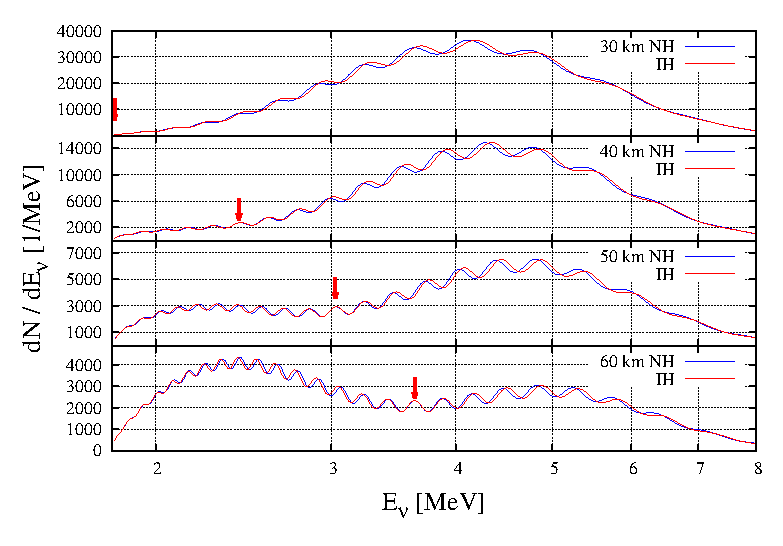
\includegraphics{figures/EventDist_combine_0.eps}
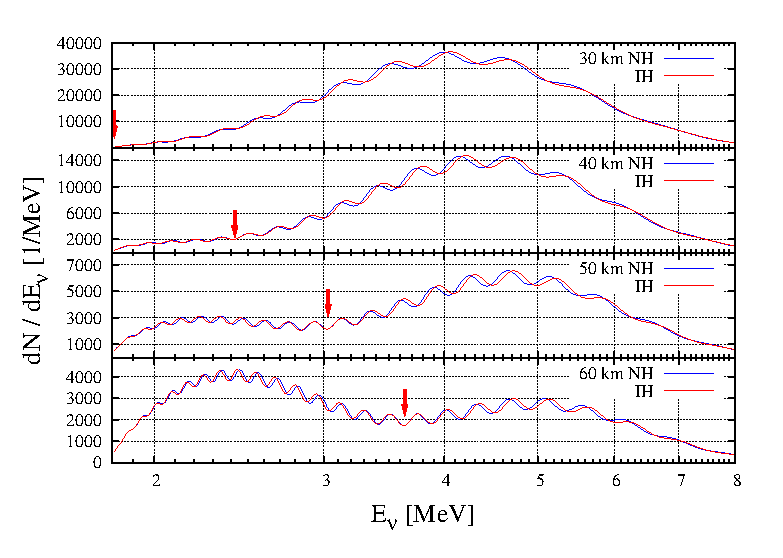
\includegraphics{figures/EventDist_combine_0_2.eps}
}
\caption{The energy distributions of reactor antineutrino events after
 \exposure\, exposure at the baseline lengths $L=30,40,50$
 and 60 km, in the top-down order. The blue curves are for NH,
 while the red ones for IH. The red arrows indicate the energies at which
 the difference due to mass hierarchy vanishes.}
\label{fig:EventDist_combine_0}
\end{figure}
There are four sets of curves for the different baseline lengths, 30, 40, 50
and 60 km, from the top to the bottom panel. In each panel, the blue and red curves show the distributions for NH and IH,
respectively. The red arrow in each
panel shows the antineutrino energy at which the mass hierarchy dependent
term, the last term in eq.~(\ref{pee2}), vanishes with $n=1$ in
eq.~(\ref{condition2}). Most of the reactor antineutrino events are expected to
populate the energy range between 1.8 MeV and
8 MeV. We note here that the difference between the NH and IH
oscillations is due to the difference of the phase $\drct$ defined in
eq.({\ref{deltaij}}), as shown in eq.(\ref{pee2}). This relative phase difference is reversed across the arrowed degeneracy point, as most clearly seen in
the $L = 60$ km case. 
%This reversal plays a crucial role in the mass hierarchy determination
%as we see in the Fig.~\ref{fig:EventDistmin_fit2nh_combine_30} and Fig.~\ref{fig:EventDistmin_fit2nh_combine_50}.

\begin{figure}[thpb]
\resizebox{0.48\textwidth}{!}{
%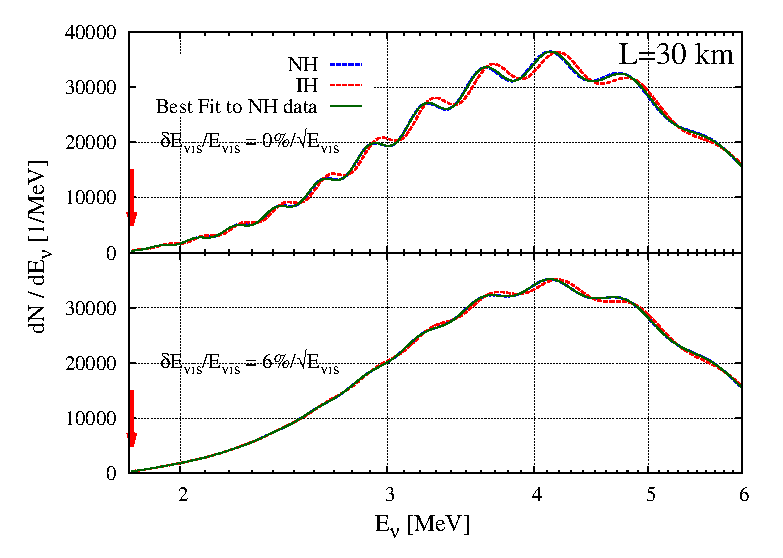
\includegraphics{figures/EventDistmin_fit2nh_combine_30.eps}
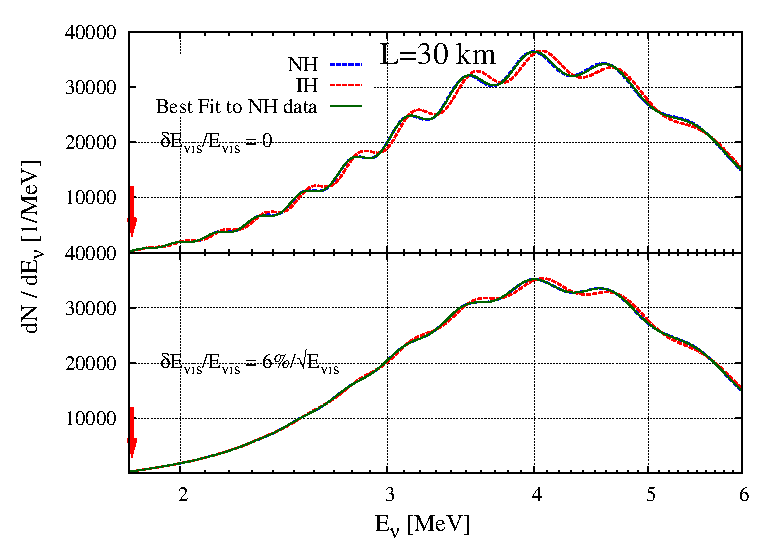
\includegraphics{figures/EventDistmin_fit2nh_combine_30_6_0.eps}
}
\caption{The energy distribution of reactor antineutrinos
 with baseline length $L = 30$ km and \exposure\, exposure. 
{\bf Upper}: The case with exact $E_{\nu}$ measurement where the dashed blue and dashed red curves are
 for NH and IH,
 respectively. The solid curve shows the
 best fit of IH assumption to the NH data.
 The red arrow points out
 the energy at which the difference due to
 mass hierarchy vanishes.
{\bf Lower}: $6/\sqrt{E_{vis}}\,\%$ energy resolution case.}
\label{fig:EventDistmin_fit2nh_combine_30}
\end{figure}

\begin{figure}[thpb]
\resizebox{0.48\textwidth}{!}{
%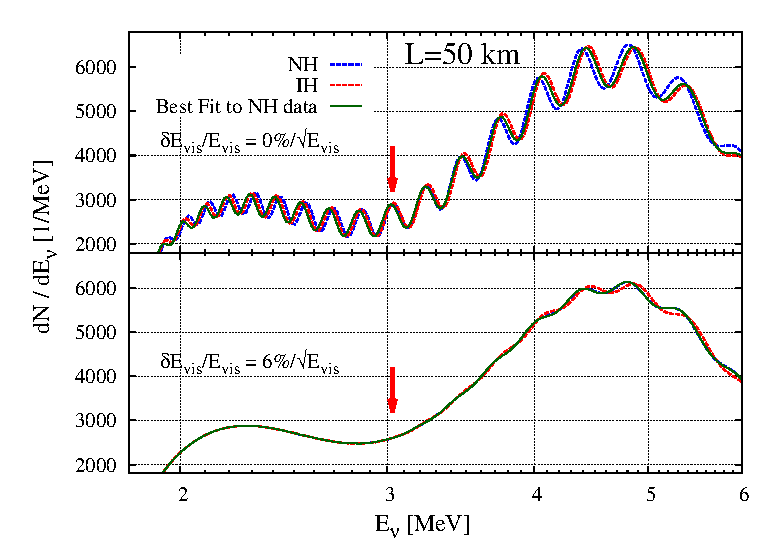
\includegraphics{figures/EventDistmin_fit2nh_combine_50.eps}
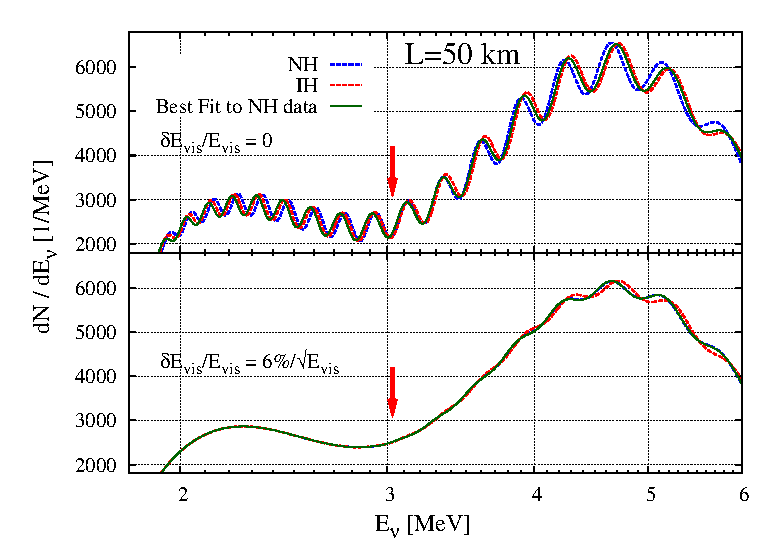
\includegraphics{figures/EventDistmin_fit2nh_combine_50_6_0.eps}
}
%\caption{Similar figure as
% Fig.~\ref{fig:EventDistmin_fit2nh_combine_30} with baseline length
% $L = 50 \mbox{km}$.}
\caption{Same as Fig.~\ref{fig:EventDistmin_fit2nh_combine_30} but with
 baseline length $L=50$ km}
\label{fig:EventDistmin_fit2nh_combine_50}
\end{figure}
Figures~\ref{fig:EventDistmin_fit2nh_combine_30}
and \ref{fig:EventDistmin_fit2nh_combine_50} show energy
distributions for $L = 30$ km and 50 km, respectively, 
in which the exact $E_{\nu}$ measurement is assumed for the upper panel, whereas in the lower
panel the energy
resolution of $a = 6\%$ with $b = 0$ in eq.~(\ref{eq:Eres}) is assumed. The dashed blue curve corresponds to
the NH case, and the dashed red curve to the IH case,
while the solid curve is obtained using the parameter values fitted to
the NH data with the ``wrong'' IH assumption. At $L = 30$ km, the solid curve
almost coincides with the dashed blue one even with the exact energy
measurement, implying that it is almost impossible to distinguish
the mass hierarchy by experiments at $L =  30$ km. This is because the
small phase shift between the NH and IH predictions can be absorbed by a
small shift in $|\dmr|$ by a fraction of its present uncertainty, $0.1
\times 10^{-3} {\rm eV}^2$.
% we will discuss this shift more
%qualitatively later. 
The situation only becomes worse with
introducing a finite energy resolution.
% This is
% simply due to the fact that the mass hierarchy difference in the energy
% distribution can be absorbed by the shift of $\dmr$ within
% its uncertainty since the relative phase between NH and IH oscillation
% almost the same in the relevant energy range of this experiment at $L
% omme=30$ km. 

The situation changes when the second peak, the $n=2$ point in eq.~(\ref{condition1}), of the mass hierarchy dependent term appears in
the energy range. The mass hierarchy difference can no longer be
absorbed by a shift in $|\dmr|$ since the relative phase difference
between the NH and IH oscillations changes across the degeneracy point.
There is no way to make the differences on the both sides compensated, 
resulting in the distinct mismatch between the dashed blue curve (for
the NH data) and the solid curve (the best-fit under the IH
assumption) as shown in the upper panel of
Fig.~\ref{fig:EventDistmin_fit2nh_combine_50}, where the antineutrino energy
is exactly measured. Once the finite energy resolution is
introduced, the phase difference in the lower energy side of the
degeneracy point is significantly smeared out as it oscillates faster w.r.t. 
$E_{\nu}$ at the low energy, hence it is easier for one oscillation
period to be covered by a sizable Gaussian profile of the detector response function. The remaining difference in the
higher energy side can then be absorbed by a small shift in $|\dmr|$,
resulting in an excellent fit (solid curve) to the NH data (blue
dashed curve) in the lower panel of
Fig.~\ref{fig:EventDistmin_fit2nh_combine_50}, shown for
$6\%/\sqrt{E/{\rm MeV}}$
energy resolution. From these result, we can conclude that the physics
potential for mass hierarchy discrimination strongly depend on the
energy resolution.
%In a word, the result has strong dependence on energy resolution.

\begin{figure}[thpb]
\resizebox{0.48\textwidth}{!}{
%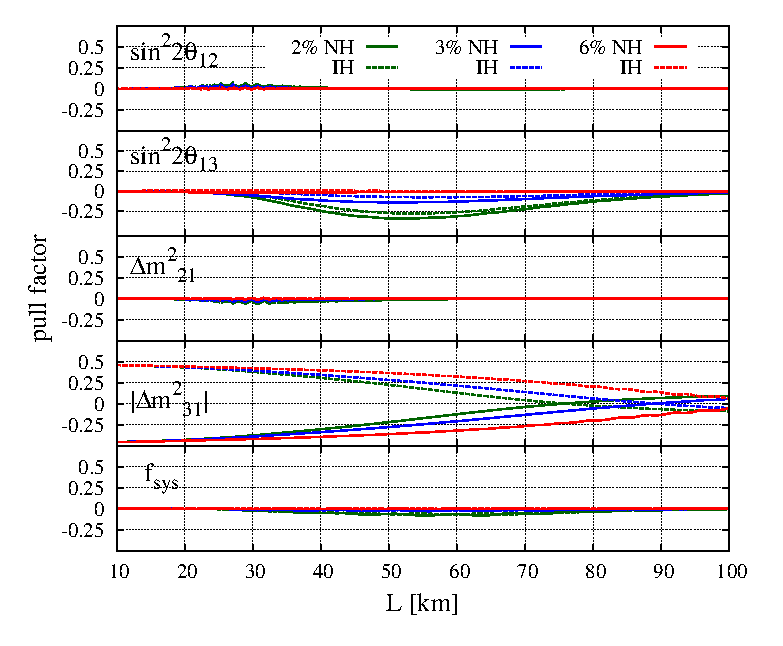
\includegraphics{figures/params.eps}
%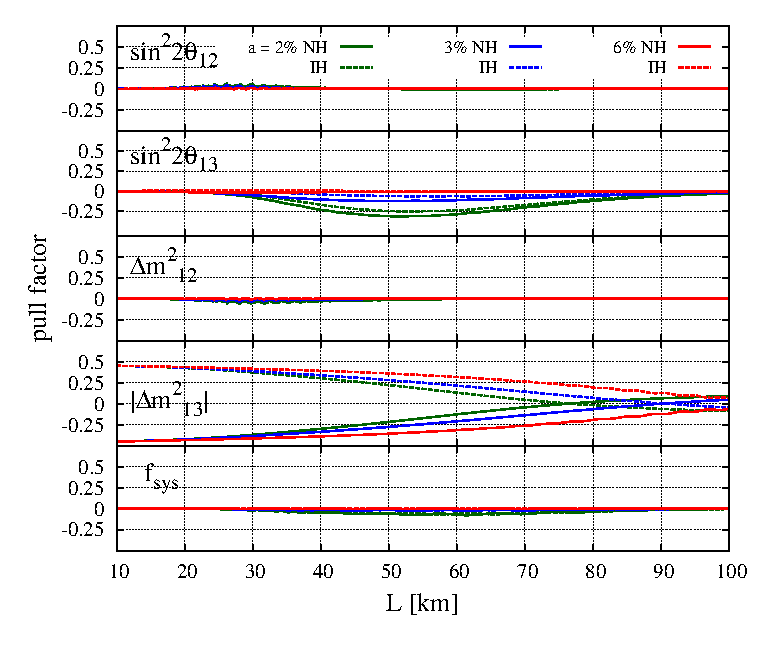
\includegraphics{figures/params_b0.eps}
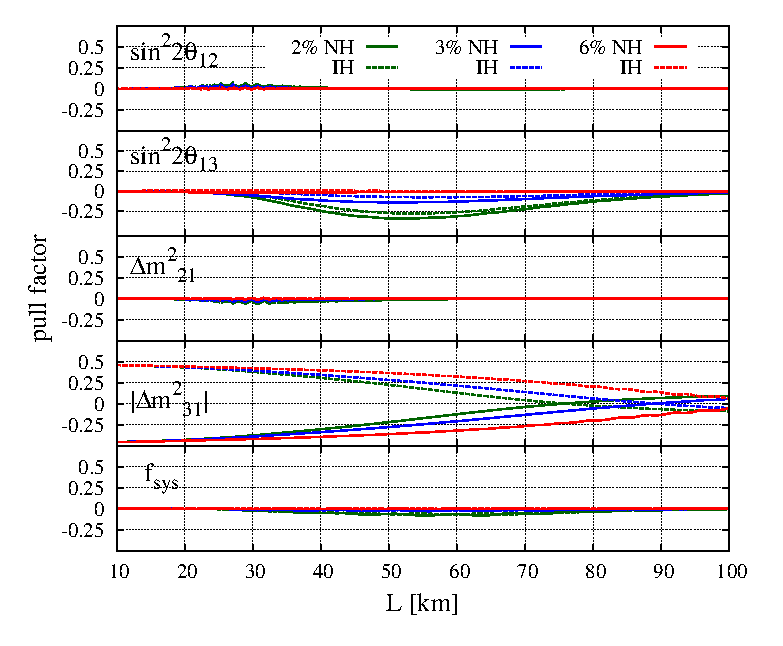
\includegraphics{figures/params.eps}
}
\caption{The best-fit values for $\ssol ,$ $\srct,$ $\dms,$ $|\dmr|$ and
 $f_{sys}$ v.s. the baseline length $L$ with $a=2\%, 3\%, 6\%$ and $b=0$. The results for \exposure\, exposure are shown by solid curves for NH, and dashed curves
 for IH.}
\label{fig:params}
\end{figure}
To discuss more qualitatively the parameter shifts which have resulted in
the excellent fits, we plot  in
Fig.~\ref{fig:params} the pull factors of the five fitting
parameters, $\ssol$, $\srct$, $\dms$, $|\dmr|$ and $f_{sys}$, as
functions of the baseline length $L$. The pull factor of parameter $Y$
is defined as $ \left(Y^{\,fit} -Y^{\,input}\right)/\delta Y$, 
and its square contributes
to the $\cT$ function of eq.(\ref{eq:chi2_func}). 
%The convention of the plots
%is the same as in Fig.~\ref{fig:dchi2_combine}, where
%$(\Delta\chi^2)_{min}$ stays almost zero at all $L$ for $a = 6\%$. 
 The best fit values with the wrong
hierarchy assumption are shown by green, blue and red curves for $a
= 2,3$ and $6\%$ with $b=0$, respectively. As expected, $|\dmr|$ shifts
significantly with a
negative (NH) or positive (IH) pull factor of 0.5 or less, especially in
short baseline lengths. 
%The tendency is similar for all the energy resolutions. 
%The amount of shift in $|\dmr|$ also depends on the energy
%resolution, smaller shifts for better resolution. This is because the
%small oscillation due to $|\dmr|$ in low energy region can be resolved more clearly in better resolution, and it becomes harder to compemsate the difference in the NH
%and IH oscillations by a
%shift in $|\dmr|$. 
Although $\srct$ also seems to contribute significantly at
$L\sim 30-80$ km for the $a=2\%$ and $3\%$ cases, we checked that its
contribution for reducing $(\dcT)_{min}$ is negligible compared to
$|\dmr|$. The other parameters do not contribute significantly. 
At large baseline length, $L > 80$ km, none of the model 
parameters gives a significant pull factor.

% To asses the rejecting power for the wrong mass hierarchy assumption more
% quantitatively, we show the $\dcT$ distribution as a function of the baseline
% length $L$ in Fig.~\ref{fig:dchi2_combine}. 
Figure~\ref{fig:dchi2_combine} shows the resulted
$(\Delta\chi^2)_{min}$ value as a function of the baseline length $L$,
for several energy resolutions, $a = 2,3,4,5$ and $6\%$ (with $b=0$) in
eq.(\ref{eq:Eres}), from the top to the bottom.
 \begin{figure}[thpb]
 \resizebox{0.48\textwidth}{!}{
% \includegraphics{figures/dchi2_qeq:Eres4.eps}
% 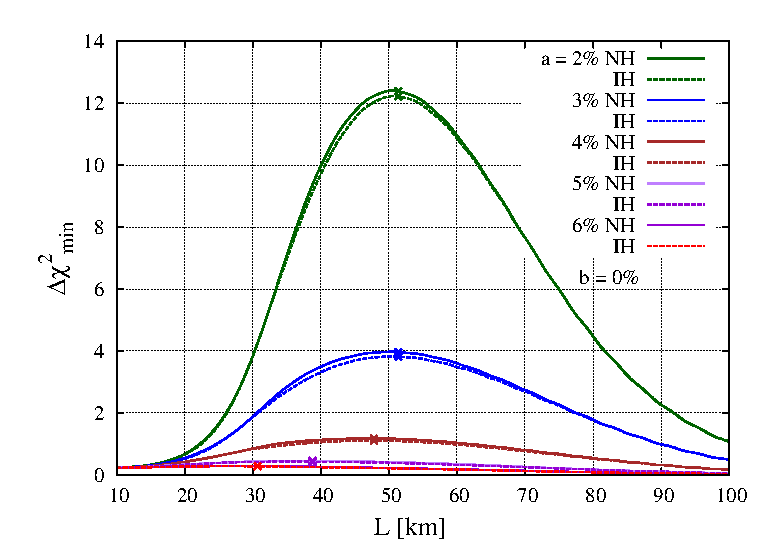
\includegraphics{figures/dchi2_combine2.eps}
 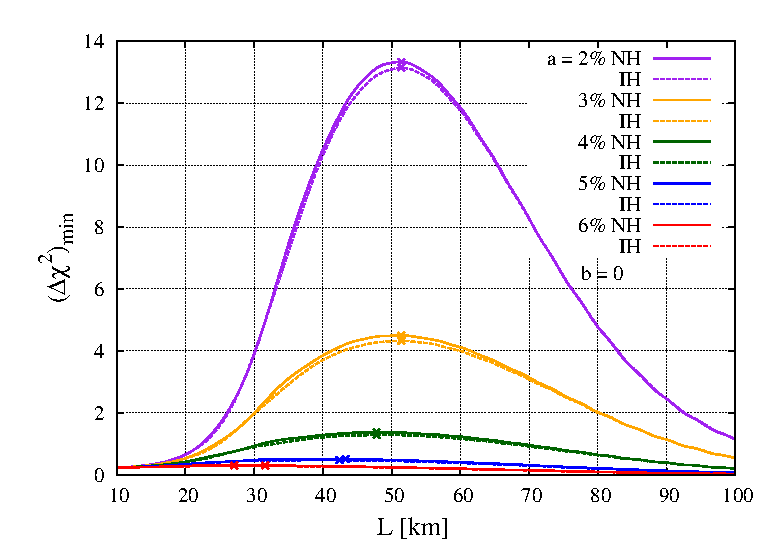
\includegraphics{figures/dchi2_combine.eps}
 }
 \caption{$(\dcT)_{min}$ for mass hierarchy discrimination shown as a function of the baseline
  length $L$, when the energy resolution in
  eq.~(\ref{eq:Eres}) is varied with $a=2$ to 6\% and $b=0$, from the top to the
  bottom. The results for \exposure\, exposure are represented by solid curves for NH, and by dashed curves for IH. The cross symbols
  mark the optimal baseline lengths.}
 \label{fig:dchi2_combine}
 \end{figure}
Solid curves are for NH, while dashed curves are for IH. The results
clearly show that the mass hierarchy can be determined by those
experiments only if the energy resolution of the detector is
$3\%/\sqrt{E/{\rm MeV}}$ or better, and that the optimal baseline length
(as shown by the cross symbol) is around 50 km for that
resolution. The small $(\dcT)_{min}$ for the baseline
length $L < 40$ km and $L>80$ km is due to a shift in $|\dmr|$ and low
statistics, respectively. For the $a=5$ and $6\%$ cases
$(\Delta\chi^2)_{min}$ stays almost zero at all $L$. 
%Our findings agree with those of
%Refs.~\cite{Learned:2006wy,Batygov:2008ku,Zhan:2008id,Zhan:2009rs,Ghoshal:2010wt,Ciuffoli:2012iz,Ciuffoli:2012bs,Qian:2012xh}
%which are obtained by the Fourier analysis, as well as those of Refs.~\cite{Petcov:2001sy,Choubey:2003qx,Batygov:2008ku,Ghoshal:2010wt,Qian:2012xh,Ghoshal:2012ju}
%that adopt the $\chi^2$ analysis similar to ours.

Next we discuss the effect of the systematic
uncertainty part of the energy resolution, $b$, in
eq.(\ref{eq:Eres}). The Fig.~\ref{fig:dchi2_2qEresnl2} shows the $(\dcT)_{min}$
value as a function of the baseline length $L$ for different $b$ values
with $a = 3\%$.
 \begin{figure}[thpb]
 \resizebox{0.48\textwidth}{!}{
% 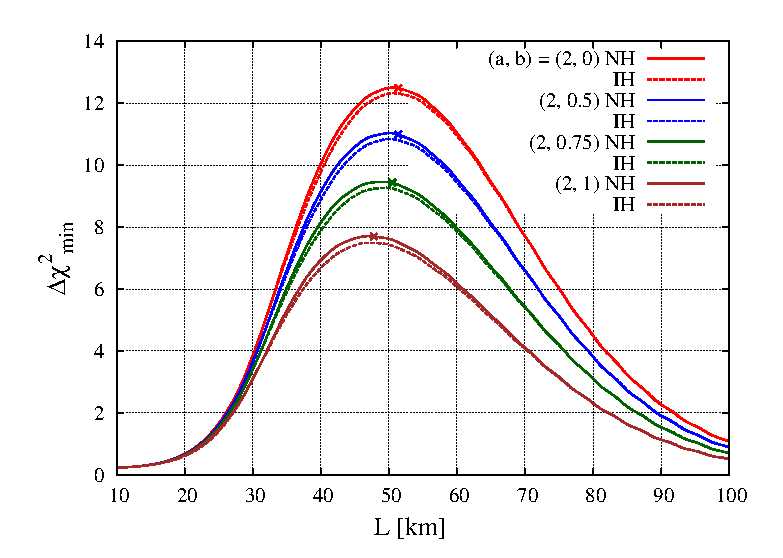
\includegraphics{figures/dchi2_2qEresnl3.eps}
% 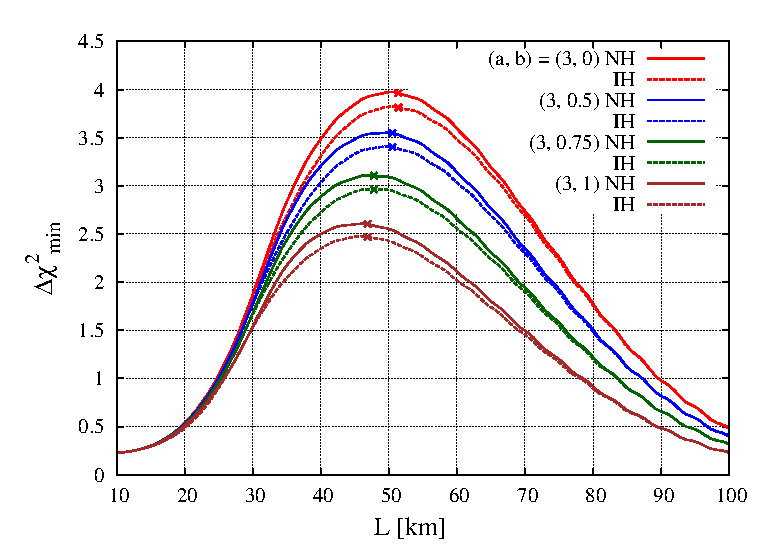
\includegraphics{figures/dchi2_3qEresnl4.eps}
 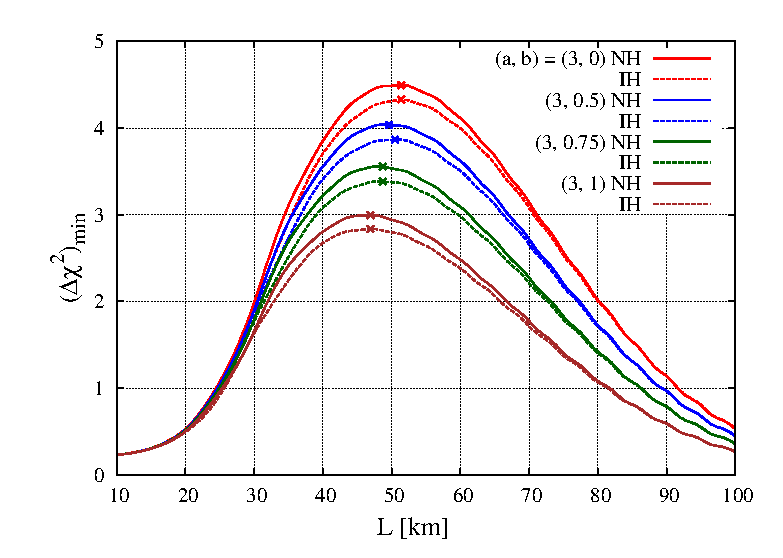
\includegraphics{figures/dchi2_combine_Eresnl_3.eps}
 }
 \caption{$(\dcT)_{min}$ for mass hierarchy discrimination v.s.
  baseline length $L$, with the energy resolution in
  eq.~(\ref{eq:Eres}) being
  $a = 3\%$ and $b = 0\%, 0,5\%, 0.75\%, 1\%$, 
  from the top to the bottom. The other conditions are the same as Fig.~\ref{fig:dchi2_combine}.}
%The results for \exposure\, exposure
%  are shown by solid curves for NH and
%  by dashed curves for IH. The cross symbols
%  show the optimal lengths of the detector that maximize $(\dcT)_{min}$.}
 \label{fig:dchi2_2qEresnl2}
 \end{figure}
 The curves from the top to the bottom are obtained for $b = 0\%, 0.5\%,
 0.75\%$ and $1\%$, respectively. The effect of the systematic uncertainty is
significant as discussed in Ref.~\cite{Qian:2012xh},
reducing the peak value of $(\dcT)_{min}$ from 4.5~($b=0$) to
 4~($b=0.5\%$), 3.5~($b=0.75\%$) and 3~($b=1\%$) for NH. 
%by a factor of up to 1.5; thus the mass hierarchy can be
% determined with 3-sigma significance only after 11-18 years running of the
% experiment for $a=3\%$ case. 
The optimal $L$ shortens
from 52 km for $(a,b) = (3,0)\%$ to 47 km for $(a,b) = (3,1)\%$. 
The Fig.~\ref{fig:dchi2_3qEresnl} shows another similar figure for
$a=2\%$.            
 \begin{figure}[thpb]
 \resizebox{0.48\textwidth}{!}{
% 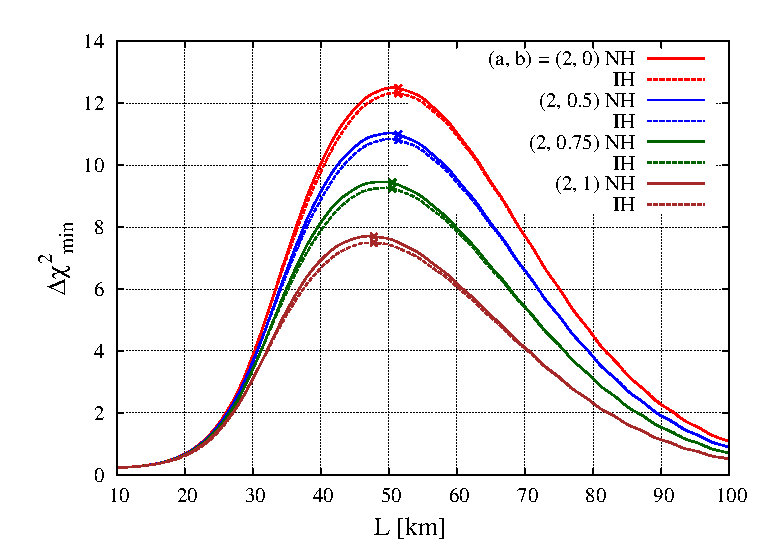
\includegraphics{figures/dchi2_2qEresnl4.eps}
 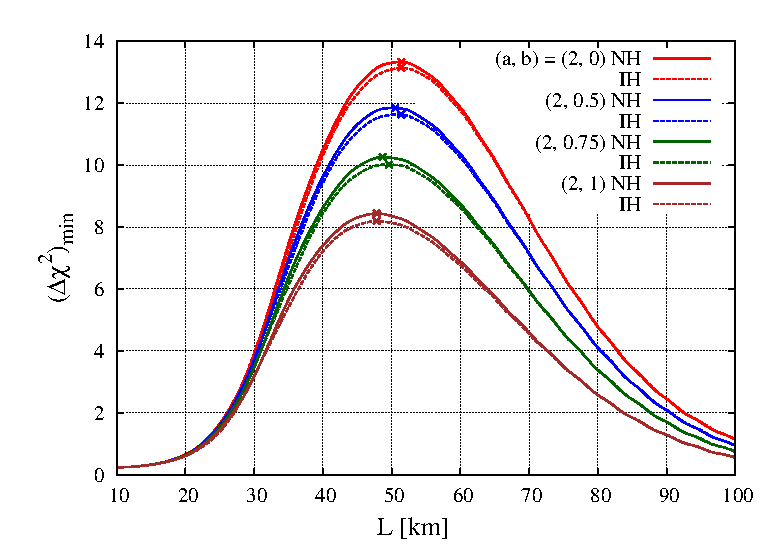
\includegraphics{figures/dchi2_combine_Eresnl_2.eps}
 }
 \caption{Same as Fig.\ref{fig:dchi2_2qEresnl2} but with the energy
  resolution $a = 2\%$ and $b = 0\%, 0.5\%, 0.75\%, 1\%$ 
  from the top to the bottom.}
 \label{fig:dchi2_3qEresnl}
 \end{figure}
 In this case $(\dcT)_{min}$ is reduced from 13.3~($b = 0$) to
 11.8~($b=0.5\%$), 10.3~($b=0.75\%$) and 8.5~($b=1\%$). 

In addition, the neutrino parameters, $\ssol, \srct, \dms$ and $|\dmr|$, can be measured accurately
with statistical uncertainties shown in
Fig.~\ref{fig:param_errors}. 
\begin{figure}[thpb]
\resizebox{0.48\textwidth}{!}{
%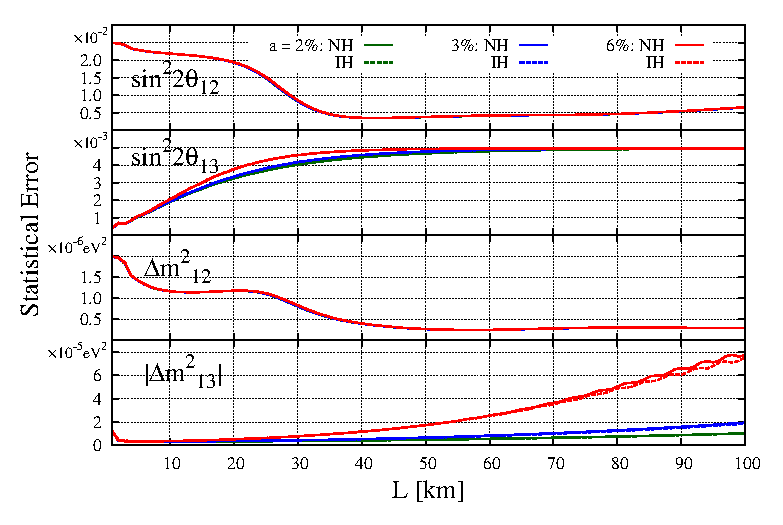
\includegraphics{figures/param_errors_b0.5.eps}
%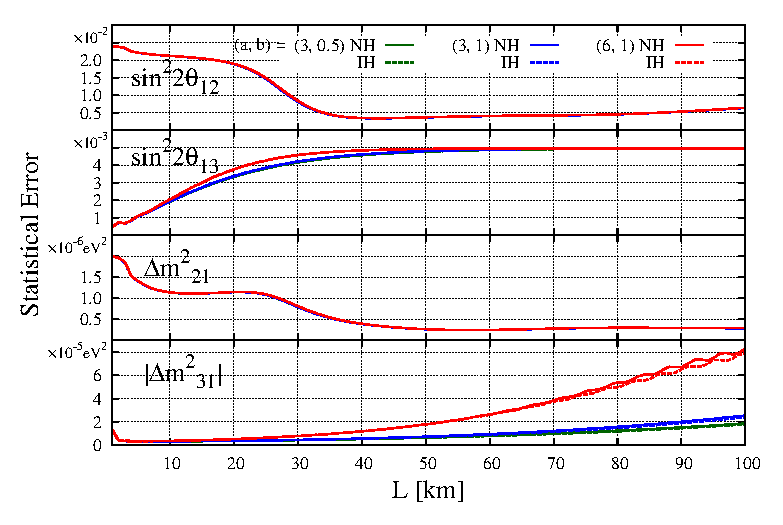
\includegraphics{figures/param_errors2.eps}
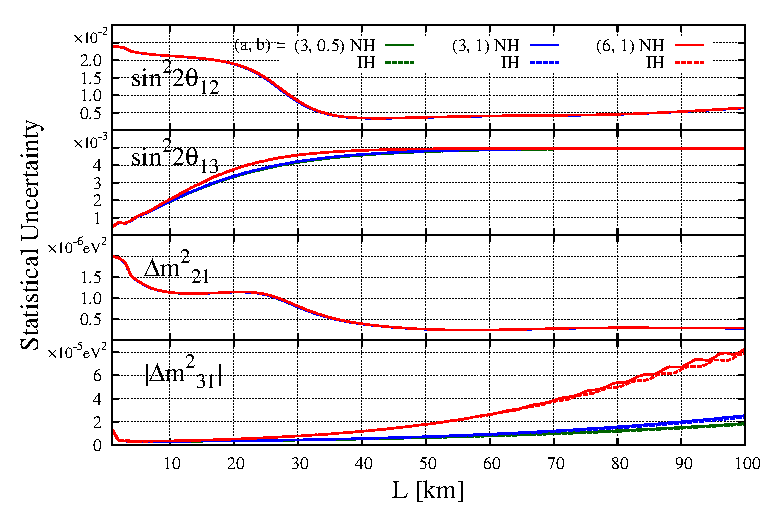
\includegraphics{figures/param_errors.eps}
}
\caption{The statistical uncertainties of the neutrino model parameters measured
 by this experiment as functions of the baseline length $L$ after \exposure\, exposure. The results for both hierarchy (NH by solid and IH by dashed
 curves) and for the energy resolution of eq.(\ref{eq:Eres}) with $(a,b)=(3,0.5),(3,1)$ and
 $(6,1)\%$ are shown.}
\label{fig:param_errors}
\end{figure}
% These
% uncertaintys are rather insensitive to the energy resolution as can be
% observed from the degeneracy even between $(a,b)=(3,0.5)\%$ and $(6,1)\%$ cases, with
% an exception of the $|\dmr|$ uncertainty for which the uncertainty grows at large
% $L$ for the $(6,1)\%$ case. 
We find
\begin{subequations}
\begin{align}
\delta\ssol \sim& 4\times 10^{-3} \,(0.5\%), \\
\delta \dms \sim& 3\times 10^{-7} {\rm eV^2} \,(0.4\%), \\
\delta |\dmr| \sim& 7\times 10^{-6} {\rm eV^2} \,(0.3\%),
\end{align}
\label{eq:param_errors}
\end{subequations}
with the energy resolution of $(a, b) = (3,0.5)\%$ at $L = 50$
km; the percentage values in the parentheses denote the relative
accuracy of the measurement. Those uncertainties are almost independent of the mass hierarchy and of
the energy resolution, with
 the only exception of the $|\dmr|$ uncertainty for which the larger resolution
 results in the larger uncertainty: $|\dmr|\sim 8\times 10^{-6} {\rm eV}^2$ for the resolution 
 $(a,b) = (3,1)\%$ and $1.8\times 10^{-5} {\rm eV}^2$ for $ (a,b) = (6,1)\%$ at $L = 50$ km. The uncertainties of $\ssol$ and $\dms$
 show the rapid reduction after $L = 20$ km and stabilize for $L > 40$
 km. This is because the normalization and shape of the slowly varying
 oscillation pattern in Fig.~\ref{fig:EventDist_combine_0} determine $\ssol$ and $\dms$, respectively, which is
 almost independent of the energy resolution. On the other hand, $\srct$
 and $|\dmr|$ are measured most accurately around $L\sim 1$ km,
 which motivated the first round of the reactor antineutrino oscillation
 experiments such as Daya Bay~\cite{DayaBay}, RENO~\cite{Ahn:2012nd} and
 Double Chooz~\cite{Abe:2011fz}. The uncertainty of $\srct$ quickly grows to
 the Daya Bay expectation of 5\%~\cite{Error_dmm31}, which is
 implemented as the input in this analysis, at $L>30$
 km. Somewhat surprisingly, the uncertainty of $|\dmr|$ remains small at the level
of $1\times 10^{-6} {\rm eV}^2$  up to $L\sim 60$ km when energy
resolution is $3\%/\sqrt{E/{\rm MeV}}$ or better. We find that this is because the
rapid oscillation pattern due to $|\dmr|$ can be resolved even after the
smearing in the observed energy as can be seen in
Fig.~\ref{fig:EventDistmin_fit2nh_combine_50}.
%, where the lower plots are
%obtained after the Gaussian smearing with the energy resolution of
%$6\%/\sqrt{E/{\rm MeV}}$. 
With better energy resolution, more oscillation patterns
are recognized and higher accuracy of the $|\dmr|$ measurement can be
achieved.
\bibliographystyle{bib/model1a-num-names}
\bibliography{bib/neutrino,bib/neutrino_c}
\end{document}
